\section{Heurística Constructiva Golosa}

\subsection{Algoritmos}

Para poder armar una heurística golosa para el problema del CIDM, en primer lugar hay que buscar un buen criterio para seleccionar que nodos pertenecerán al cubrimiento, dado los nodos que ya han sido agregados.

\subsubsection{Por grado}

Al principio decidimos implementar esta heurística utilizando un heap, ordenando los nodos por su grado. Luego, desencolamos del heap y vamos actualizando los flags de cada nodo a medida que son alcanzables. El algoritmo tiene \order{n \times log(n) + m}.

\subsubsection{Scoring}

Aunque este método con el heap es rápido, en realidad podemos mejorar la forma en la que seleccionamos los vértices. Este método consiste en tomar el numero de nodos adyacentes efectivos (score) a los que cada nodo puede acceder. Definimos a un nodo adyacente efectivo como un nodo que es adyacente y a su vez no puede ser accedido por otros nodos que ya pertenecen a la solución parcial en construcción. De esta forma, este criterio también nos garantiza la independencia del conjunto, dado que si tomamos dos nodos de la solución, por construcción no pueden ser adyacentes.

Cada nodo va a tener como atributos su score, un flag que indica si ha sido agregado y otro que indica si es alcanzable por el cubrimiento parcial actual.

El algoritmo va a iterar un arreglo de nodos $n^2$ veces. Cada vez que busquemos un nodo para agregar al conjunto, los iteraremos todos para buscar el de máximo score. Al identificarlo, actualizaremos los scores de los nodos adyacentes a los adyacentes del mismo. A priori parece que la complejidad de este nuevo algoritmo se podría mejorar de forma significativa utilizando algún otro tipo de estructura de datos.

\subsection{Complejidad}

El primer algoritmo resuelve el problema en \order{n \times log(n) + m} simplemente ignorando la actualización de los scores, desencolando de un heap $n$ veces. Sin embargo, este criterio es a simple vista inferior que el de actualización de scores. Aquí hay un tradeoff entre hacer la mejor elección y la complejidad temporal del algoritmo.

El algoritmo basado en el score recorre arreglo $n$ veces. A su vez, buscar los adyacentes de los adyacentes se hace $m$ veces. Luego actualizamos en total el score de $m$ nodos. Por lo tanto, el algoritmo tiene orden \order{n^2 + 2 \times m}.

Notar que la forma en que buscamos el máximo es sumamente ineficiente. Esto se debe a que si utilizamos sort, luego es bastante difícil encontrar el nodo al que le debemos actualizar su respectivo score. A su vez, dado que en cada iteración actualizamos el score, mantener el orden es sumamente costoso. Es muy posible que exista una estructura de datos mucho mas eficiente para resolver este problema (una especie de heap dinámico). Knuth \footnote{El rey de las estructuras de datos.} seguramente nos querría pegar.

\pagebreak

\subsection{Efectividad de la heurística}

Nuestra heurística no siempre devuelve la solución optima. Considerar los siguientes ejemplos:

\begin{figure}[ht]
\centering
\begin{subfigure}[b]{0.4\textwidth}
	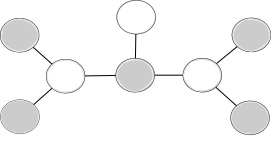
\includegraphics[scale=0.6]{images/greedy_fail.png}
	\caption{Greedy (5 nodos)}
\end{subfigure}
\begin{subfigure}[b]{0.4\textwidth}
	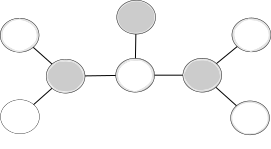
\includegraphics[scale=0.6]{images/greedy_best.png}
	\caption{Optimo (3 nodos)}
\end{subfigure}

\begin{subfigure}[b]{0.4\textwidth}
	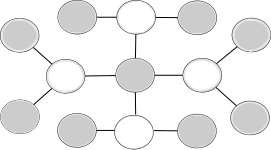
\includegraphics[scale=0.6]{images/greedy_fail2.png}
	\caption{Greedy (9 nodos)}
\end{subfigure}
\begin{subfigure}[b]{0.4\textwidth}
	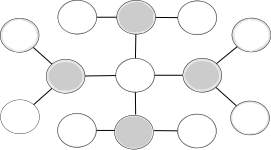
\includegraphics[scale=0.6]{images/greedy_best2.png}
	\caption{Optimo (4 nodos)}
\end{subfigure}
\caption{Ejemplos de nuestra heurística comparado con el optimo.}
\end{figure}

El peor caso es claramente el de la figura (c) y (d). Tenemos un nodo $v$ de grado $d(v) = n$, con sus nodos adyacentes de grado $d(u) = n - 1$. Si tenemos $c$ componentes conexas de ese tipo, utilizaremos $c \times (n \times (n-2) + 1)$ nodos, cuando en realidad el optimo tiene $c \times n$ nodos.



